\documentclass[a4paper]{article}
\usepackage[utf8]{inputenc}
\usepackage[spanish, es-tabla, es-noshorthands]{babel}
\usepackage[table,xcdraw]{xcolor}
\usepackage[a4paper, footnotesep = 1cm, width=20cm, top=2.5cm, height=25cm, textwidth=18cm, textheight=25cm]{geometry}
%\geometry{showframe}

\usepackage{tikz}
\usepackage{amsmath}
\usepackage{amsfonts}
\usepackage{amssymb}
\usepackage{float}
\usepackage{graphicx}
\usepackage{caption}
\usepackage{subcaption}
\usepackage{multicol}
\usepackage{multirow}
\setlength{\doublerulesep}{\arrayrulewidth}
\usepackage{booktabs}

\usepackage{hyperref}
\hypersetup{
    colorlinks=true,
    linkcolor=blue,
    filecolor=magenta,      
    urlcolor=blue,
    citecolor=blue,    
}

\newcommand{\quotes}[1]{``#1''}
\usepackage{array}
\newcolumntype{C}[1]{>{\centering\let\newline\\\arraybackslash\hspace{0pt}}m{#1}}
\usepackage[american]{circuitikz}
\usetikzlibrary{calc}
\usepackage{fancyhdr}
\usepackage{units} 

\graphicspath{{../Calculos-Potencia/}{../Caracteristicas/}{../Consideraciones/}{../Gain-Stage/}{../Input-Stage/}{../Output-Stage/}{../Simulaciones/}{../Alimentacion/}{../Conclusiones/}}

\pagestyle{fancy}
\fancyhf{}
\lhead{22.12 Electrónica II}
\rhead{Mechoulam, Lambertucci, Rodriguez, Londero, Scala}
\rfoot{Página \thepage}

\begin{document}

\tableofcontents
\newpage
%%%%%%%%%%%%%%%%%%%%%%%%%%%%%%%%%%%%%%%%%%%%%%%%%%%%%%%%%%%%%%%%%%%%%%
\subsection{Diseño Propuesto}

En la siguiente instancia se realiza una fuente de tensión regulada, la cual se ajusta a las especificaciones de:
\begin{align*}
	0 \ V \leq V_o \leq 9 \ V \\
	I_{o-Max}=2.5 \ A
\end{align*}

Se optó por un diseño que muestre tensión y sume corriente, siendo el diseño elegido para la fuente el presentado a continuación.
\begin{figure}[H]
\centering
	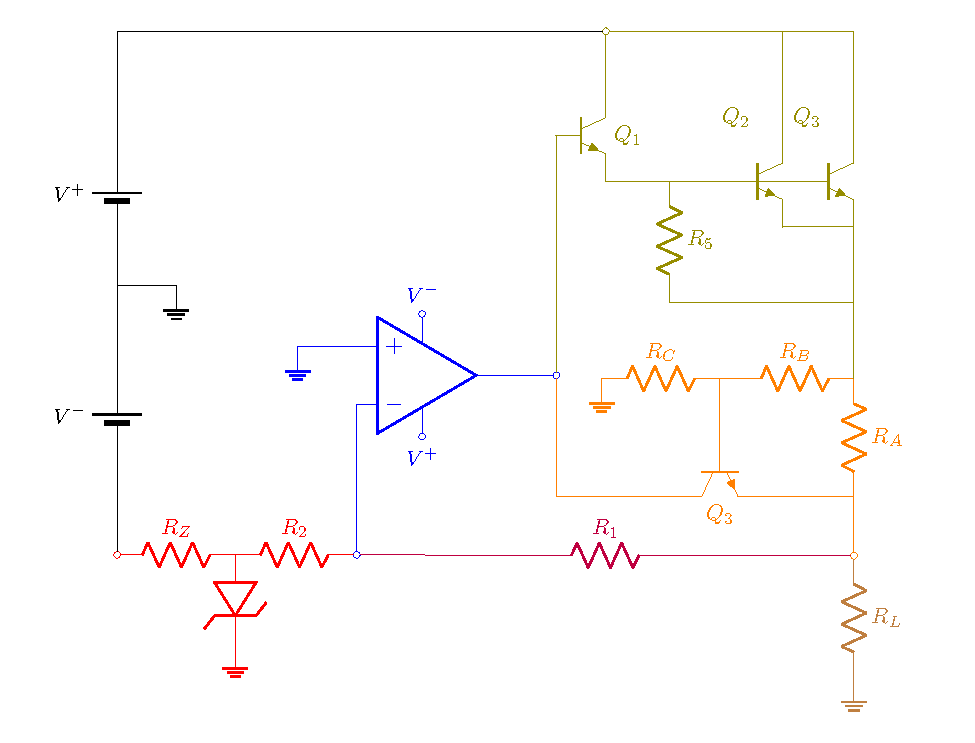
\includegraphics[width=0.8\textwidth, page=1]{ImagenesEjercicio2/Regulador.pdf}
	\caption{Circuito regulador de tensión propuesto.}
	\label{fig:circuitoprop}
\end{figure}

Dicho circuito puede ser separado en 5 bloques fundamentales:
\begin{itemize}
\item \textcolor{blue}{Amplificador error}
\item \textcolor{olive}{Transistor de paso}
\item \textcolor{red}{Elemento de referencia}
\item \textcolor{purple}{Circuito de detección}
\item \textcolor{orange}{Circuito de protección}
\end{itemize}

\subsubsection{Análisis de realimentación negativa}
\label{sec:realimentacion-negativa}

La teoría de la realimentación negativa plantea que dado un sistema a lazo cerrado ideal, con un número impar de inversiones de fase, la ganancia de este puede aproximarse como la inversa del factor de realimentación si la ganancia de lazo en módulo es mucho mayor a la unidad, es decir
\begin{equation}
P.E. = \frac{A }{1+ f \cdot A} = \frac{1}{f} \cdot \frac{|T|}{1 + |T|}
\end{equation}
donde $A$ es la respuesta a lazo abierto, $f$ el factor de realimentación y $T$ es la ganancia de lazo. Se puede observar que bajo las condiciones descritas anteriormente, se tiene entonces que 

\begin{equation}
P.E. \approx \frac{1}{f}
\end{equation}

\begin{figure}[H]
\centering
	\includegraphics[width=0.8\textwidth, page=4]{ImagenesEjercicio2/Regulador.pdf}
	\caption{Lazo de realimentación negativa.}
	\label{fig:circuito_lazo}
\end{figure}

En el circuito realizado puede observarse un lazo de realimentación negativa el cual posee una inversión de fase producida por el amplificador operacional detallado en la Figura (\ref{fig:circuito_lazo}). También es de interés observar los siguientes puntos: 
\begin{itemize}
\item Por tierra virtual, el opamp trabaja para mantener la tensión nula en su terminal negativo.
\item El diodo zener consume la corriente necesaria para mantener la caída de tensión sobre este fija.
\item El lazo de realimentación trata de fijar una tensión a la salida de la fuente regulada.
\end{itemize}

Teniendo en cuenta dichos aspectos, es de notar que la fuente realiza un muestreo de tensión a la salida mediante la resistencia $R_1$, la cual inyecta una corriente proporcional a la dicha, realizándose una suma de corrientes en el nodo del terminal negativo del amplificador operacional, siendo la referencia la corriente fija proporcionada por la resistencia $R_2$.

En resumidas cuentas, el parámetro estabilizado del sistema es

\begin{equation}
P.E. = \frac{V_o}{I_N} = -\frac{V_o \cdot R_2}{|V_z|} = \frac{1}{f} \cdot \frac{|T|}{1 + |T|}
\end{equation}

Luego, se puede demostrar que la ganancia $f$ se puede aproximar como la razón entre el parámetro que se suma en el lazo y el parámetro que se muestrea, cuando la tensión en el nodo del terminal negativo del opamp es cero, obteniendo así
\begin{equation}
f \approx -\frac{1}{R_1}
\end{equation}

Si se considera que la ganancia de lazo en módulo es mucho mayor que la unidad dado que se utiliza un opamp como amplificador, se obtiene finalmente que
\begin{equation}
V_o = |V_z| \cdot \frac{R_1}{R_2}
\label{eq:vovz}
\end{equation}

\subsection{Bloques del Regulador}
\subsubsection{Elemento de Referencia}

El elemento de referencia (o también llamado entrada o generador en un circuito de realimentación negativa) proporciona la tensión de entrada al sistema, la cual comparte nodo con el amplificador error y el circuito de detección, como se mencionó anteriormente.

En cuanto al funcionamiento, el zener está polarizado por $V^{-}$ y $R_Z$. Esta etapa del sistema es prácticamente independiente del resto del circuito, y además debe ser altamente estable, es por ello que se utiliza $R_Z >> r_Z$ para evitar variaciones de $V_Z$, es decir, de la tensión de referencia, con respecto a $V^{-}$. Para ello se plantea las ecuaciones propias del nodo $V_Z$: 
\begin{figure}[H]
\centering
	\includegraphics[width=0.5\textwidth, page=6]{ImagenesEjercicio2/Regulador.pdf}
	\caption{Circuito de transistor de paso.}
	\label{fig:transistorDePaso}
\end{figure}

\begin{equation*}
	\frac{V^{-} - V_Z}{R_Z} + I_Z = \frac{V_Z - V_1}{R_2} \approx \frac{V_Z}{R_2}
\end{equation*}
\begin{equation*}
	V^{-} - V_Z = \left( \frac{V_Z}{R_2} - I_Z \right) \cdot \frac{1}{R_Z}
\end{equation*}
\begin{equation}
	R_Z = R_2 \cdot \frac{V^{-} - V_Z}{V_Z - R_2 I_Z}
	\label{eq:referencia}
\end{equation}

\subsubsection{Circuito de Detección}
\label{sec:circuito-de-deteccion}

El circuito de detección está compuesto por la resistencia $R_1$. La caída de potencial sobre esta depende solamente de la tensión a la salida de la fuente, lo que permite generar una corriente proporcional a esta.
\begin{figure}[H]
\centering
	\includegraphics[width=0.5\textwidth, page=7]{ImagenesEjercicio2/Regulador.pdf}
	\caption{Circuito de detección.}
	\label{fig:circdeteccion}
\end{figure}

De esta manera, se genera una resta de corrientes en el nodo del terminal negativo del operacional, siendo estas la corriente suministrada por la $R_2$, la corriente fija suministrada por la $R_1$ y la corriente del terminal negativo del opamp. Se denomina a esta última corriente como el error de la fuente regulada.

\subsubsection{Amplificador de Error y Pre-regulador}
\label{sec:amp-error}

\begin{figure}[H]
\centering
	\includegraphics[width=0.8\textwidth, page=8]{ImagenesEjercicio2/Regulador.pdf}
	\caption{Corrientes en circuito de detección, elemento de referencia y operacional.}
	\label{fig:amp-prereg-det-ref}
\end{figure}

En la Sección (\ref{sec:circuito-de-deteccion}) se analizó como se genera una resta de corrientes en el nodo del terminal negativo del operacional. Se observa que, si se define a la corriente $i_1$ como la corriente suministrada por la resistencia $R_1$, la cual depende de la tensión fija impuesta por el zener, la corriente $i_2$ como la corriente suministrada por la resistencia $R_2$, la cual depende de la tensión que efectivamente provee la fuente regulada, e $i_e$ como la corriente error que atraviesa el terminal negativo del operacional, se tiene que
\begin{equation}
	i_e = i_1 - i_2 = \frac{V_o}{R_1} - \frac{-V_z}{R_2}
\end{equation}

Esta corriente error es amplificada por el operacional para luego ser inyectada a la base del transistor de paso, lo cual aumenta (o disminuye) la tensión a la salida de la fuente regulada, mitigando la corriente de error. Si se da la situación que $i_e = 0$, se observa el resultado obtenido en la Sección (\ref{sec:realimentacion-negativa}) dado que
\begin{equation}
V_o = |V_z| \cdot \frac{R_1}{R_2}
\end{equation}

Es por ello que el amplificador operacional amplifica el error de la fuente regulada y además entrega la corriente necesaria a la base del transistor de paso.

\subsubsection{Transistor de Paso}

\label{sec:transistor-de-paso}
El transistor de paso se encarga de llevar a cabo las correcciones detectadas por el circuito de detección y amplificadas por el amplificador de error, proveyendo así la corriente necesaria para mantener la diferencia de potencial fija a la salida. Este bloque se puede implementar con un par Darlington integrado, el cual tiene una gran ganancia de corriente, pero en este caso se implementa con un Darlington discreto, el cual debe soportar una corriente y potencia elevada, lo cual se profundiza más adelante en el informe. Por estas razones, se optó por utilizar dos transistores en paralelo para el segundo transistor del par, con la idea de dividir la carga de la siguiente manera:
\begin{figure}[H]
\centering
	\includegraphics[width=0.5\textwidth, page=5]{ImagenesEjercicio2/Regulador.pdf}
	\caption{Circuito de transistor de paso.}
	\label{fig:transistorDePaso}
\end{figure}
siendo $Q_2$ y $Q_3$ transistores de potencia. Por otro lado, la función de $R_5$ es obtener una corriente de colector de $Q_1$ razonable.

\subsection{Protección por Corto-circuito}
Implementar una protección de cortocircuito es una sección fundamental en el diseño de una fuente de tensión debido que no se conoce con exactitud que carga va a ser proporcionadas al circuito, como puede ser el caso de que el usuario, en contra-indicación de las especificaciones del equipo, utilice una carga menor a la mínima. En dicha situación, es deseable que el circuito no sufra un daño irreversible. Es por ello que se evaluaron 2 alternativas, las cuales son presentadas a continuación.
\subsubsection{Protección Lineal}
La implementación de una protección lineal resulta ser la mas sencilla debido a la facilidad de cálculo y que utiliza pocos componentes, como se ve a continuación:
\begin{figure}[H]
\centering
	\includegraphics[width=0.5\textwidth, page=3]{ImagenesEjercicio2/Regulador.pdf}
	\caption{Circuito de Protección lineal.}
	\label{fig:circuitolineal}
\end{figure}
El cálculo para la resistencia es simple, siendo este 
$$R_a= \frac{V_{BE}}{I_{o-Max}}$$
Esta protección limita la corriente de salida del regulador haciéndola constante. Esto es así debido a que el transistor de protección se encuentra censando la tensión sobre la resistencia $R_a$. Al superar cierto valor $V_a = R_a I_{o-Max}$ el transistor pasa a modo activo directo, quitándole corriente de la base al de paso. Es por ello que cuenta con la siguiente característica:
\begin{figure}[H]
\centering
	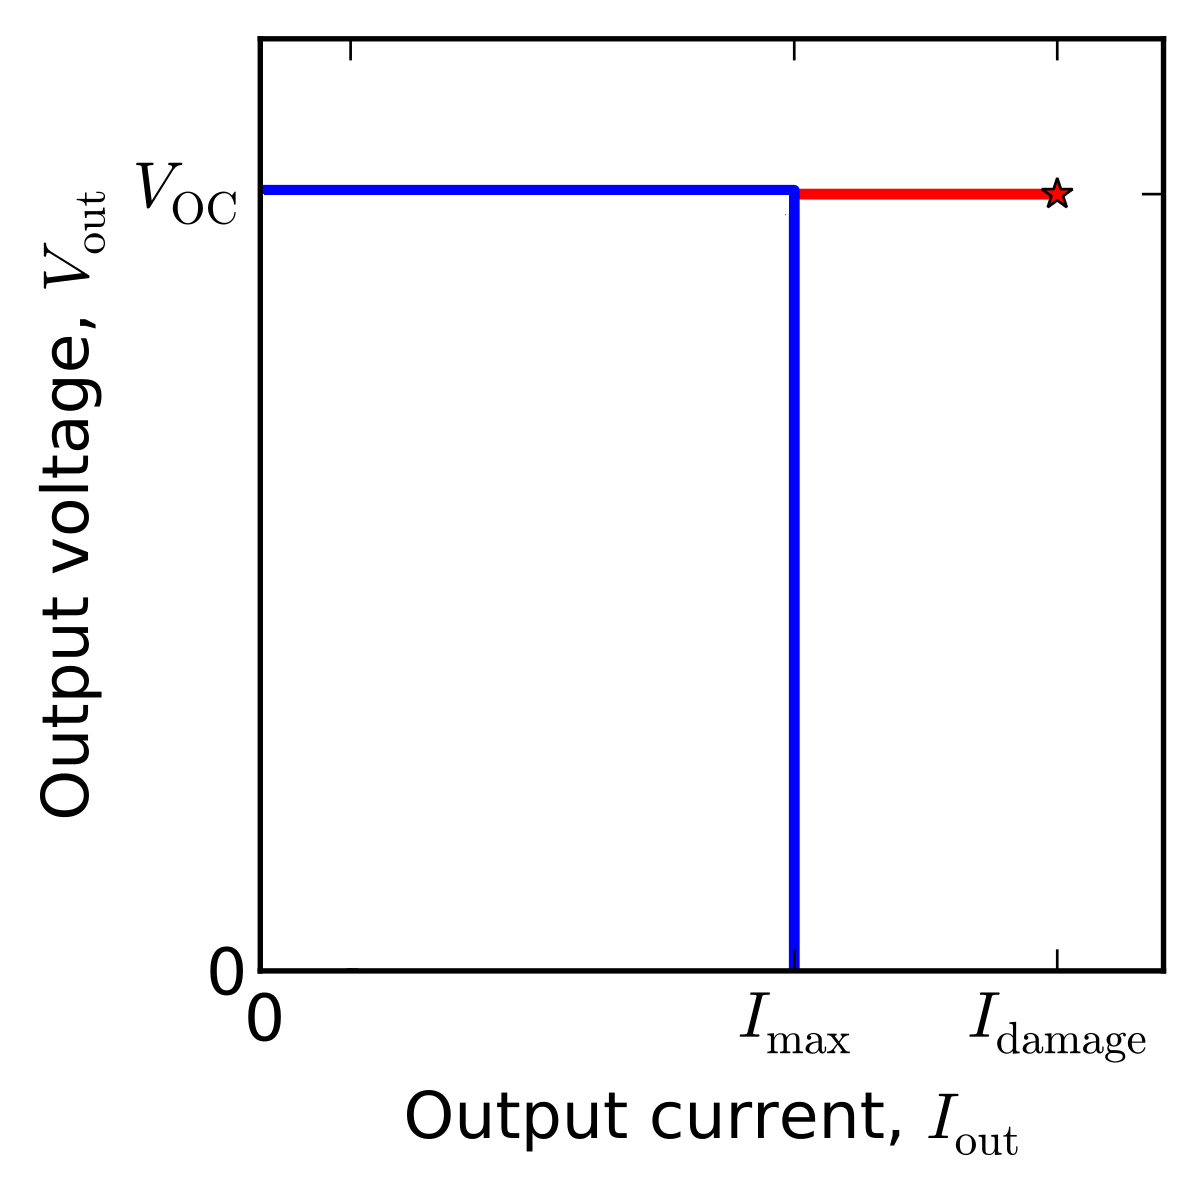
\includegraphics[width=0.4\textwidth]{ImagenesEjercicio2/Linearprotection.png}
	\caption{Característica de la protección Lineal.}
	\label{fig:circuitolinealcarac}
\end{figure}
En la Figura (\ref{fig:circuitolinealcarac}) se observa que $I_{max}$ corresponde a la máxima corriente que uno define para el circuito, mientras que $I_{damage}$ es la corriente bajo la cual el circuito sufre un daño irreversible.

Se puede notar que en el peor caso ($V_o = 0$), la corriente de salida, como la caída de potencial sobre el transistor de paso, son máximas, haciendo que también sea máxima la disipación de potencia sobre este.

\subsubsection{Protección Foldback}
La protección de Foldback es una variación de la lineal, la cual cuenta con 2 resistencias adicionales conectadas de la siguiente manera:
\begin{figure}[H]
\centering
	\includegraphics[width=0.5\textwidth, page=2]{ImagenesEjercicio2/Regulador.pdf}
	\caption{Circuito de Protección Foldback.}
	\label{fig:circuitofoldback}
\end{figure}
Si se desea resolver para $I_{o-Max}$ basta con recorrer la malla:
\begin{align}
-I_{o-Max} \cdot R_a + V_{BE} - (V_b-V_a)=0
\end{align}
\begin{align}
V_b=V_a \cdot \frac{R_c}{R_c+R_b}
\end{align}
\begin{align}
-I_{o-Max} \cdot R_a + V_{BE} + V_a \cdot (1-\frac{R_c}{R_c+R_b})=0
\end{align}
\begin{align}
-I_{o-Max} \cdot R_a + V_{BE} + (I_{o-Max} \cdot R_a +V_o) \cdot \frac{R_b}{R_c+R_b}=0
\end{align}
lo cual despejando para $I_{o-Max}$ queda:
\begin{align}
I_{o-Max}=  \frac{V_o \cdot R_b + V_{BE}\cdot (R_b+R_c)}{R_a \cdot R_c}
\label{eq:Imaxfoldback}
\end{align}

De aquí se puede ver que la corriente cae en función de la tensión de salida hasta establecerse en una corriente fija para la carga nula denominada $I_{sc}$.
\begin{align}
I_{sc} = V_{BE} \cdot \frac{R_b+R_c}{R_a \cdot R_c}
\label{eq:Isc}
\end{align}

Graficando la curva se obtiene:
\begin{figure}[H]
\centering
	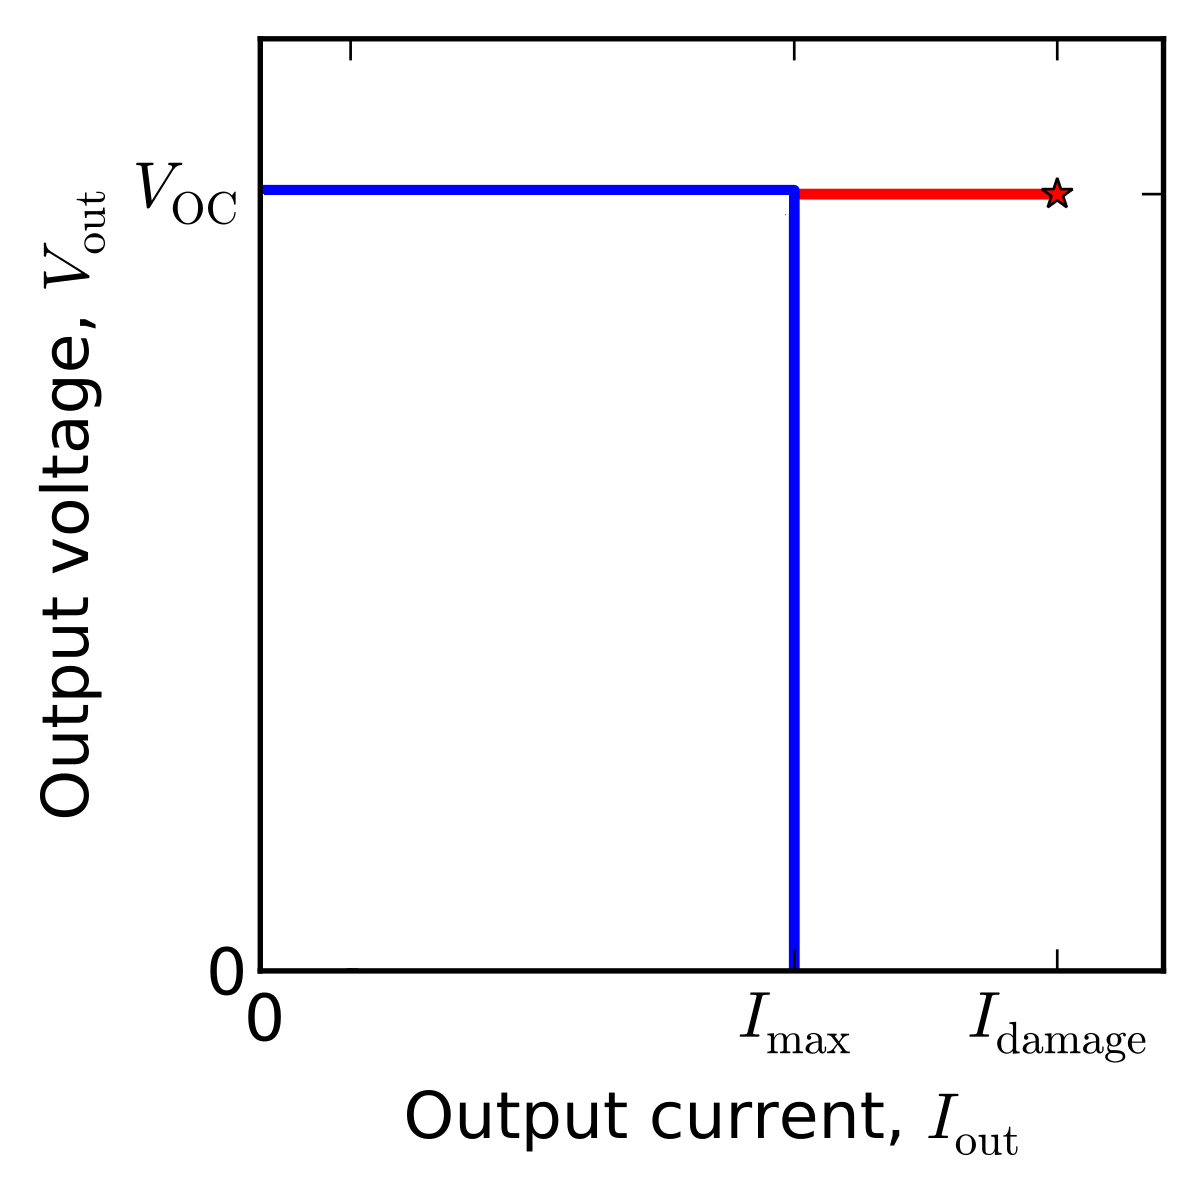
\includegraphics[width=0.4\textwidth]{ImagenesEjercicio2/foldbackLineal.png}
	\caption{Característica de la protección Foldback.}
	\label{fig:circuitofoldbackcarac}
\end{figure}
Se puede apreciar la razón de su nombre dado que la curva de la corriente se ``dobla'' sobre si misma. Si bien armar esta fuente resulta en una mayor cantidad de componentes, el hecho de que reduzca la corriente de paso al tener una carga nula, y que por ello reduzca la potencia consumida, es un factor no menor. Por dicha razón, esta fue la protección elegida para el diseño. A modo ilustrativo se grafica ambas curvas de las protecciones superpuestas.
\begin{figure}[H]
\centering
	\includegraphics[width=0.4\textwidth]{ImagenesEjercicio2/foldback.png}
	\caption{Característica de la protección Foldback y Lineal.}
	\label{fig:circuitofoldbacklinealcarac}
\end{figure}

%%%%%%%%%%%%%%%%%%%%%%%%%%%%%%%%%%%%%%%%%%%%%%%%%%%%%%%%%%%%%%%%%%%%%%
\subsection{Análisis de Componentes}
\subsubsection{Amplificador Operacional}
En la elección del amplificador operacional, se analizaron diversos componentes, siendo estos los presentados a continuación en el siguiente cuadro comparativo:
\begin{table}[H]
\hspace*{-0.5cm}
\begin{tabular}{ccccccccc}
\hline
\textbf{Amplificador Operacional} & \textbf{GBP [Mhz]} & $\mathbf{SR [\frac{V}{\mu s}]}$ & $\mathbf{Z_{in} [\Omega]}$ & $\mathbf{Z_{out}[\Omega]}$ & $\mathbf{I_{bias}[A]}$ & $\mathbf{I_{off}[A]}$ & $\mathbf{V_{off}[mV]}$ & \textbf{THD} \\ \hline
\href{http://www.ti.com/lit/ds/symlink/tl082-n.pdf}{TL082}                   & 3                  & 13                              & 1T                         & -                          & 30p                 & 5p                    & 3                      & 0.003$\%$    \\
\href{http://www.ti.com/lit/ds/symlink/lm324-n.pdf}{LM324}                    & 1                  & 0.3                             & -                          & -                          & 45n                  & 5n                     & 2                      & -            \\
\href{http://www.ti.com/lit/ds/symlink/lm833.pdf}{LM833}                    & 10                 & 5                               & -                          & 37                         & 300n                & 10n                   & 0.3                    & 0.002$\%$    \\
\href{http://www.ti.com/lit/ds/symlink/lf356-mil.pdf}{LF356}                    & 2.5                & 12                              & 1T                         & -                          & 20p                 & 50p                   & 3                      & -            \\
\href{https://www.alldatasheet.com/datasheet-pdf/pdf/49039/AD/OP284.html}{OP284}                    & 4.25                & 4                              & -                         & 210 & 60n                 & 2n                   & 125m                      & $\leq 0.005\%$           \\
\href{http://www.ti.com/lit/ds/symlink/lm741.pdf}{LM741}                    & 1.5                & 0.5                             & 2M                         & 75                         & 80n                 & 20n                   & 2                      & -            \\
\href{http://www.ti.com/lit/ds/slos070d/slos070d.pdf}{NE5534}                   & 10                 & 13                              & 100k                       & 0.3                        & 500n                & 20n                   & 0.5                    & -           \\
\hline
\end{tabular}
\caption{Comparación de operacionales.}
\end{table}

Es notable que de todos los integrados el OP284 es rail to rail, lo cual es de gran utilidad si se desea obtener un valor de $V_1$ inferior. Además, se tuvo en cuenta el GBP, las corrientes de bias, la tension de offset, para optar utilizar el OP284.

\subsubsection{Transistores de Paso}

Para la sección de transistor de paso, se eligió utilizar los transistores \href{https://pdf1.alldatasheet.com/datasheet-pdf/view/532914/FAIRCHILD/TIP31C.html}{QTIP41C} que son transistores de potencia, al igual que un \href{https://pdf1.alldatasheet.com/datasheet-pdf/view/2895/MOTOROLA/BC547C.html}{BC547C}, utilizando los TIP41C como el transistor por el cual pasará la mayoría de la corriente y el BC547 como el que recibe la corriente del opamp.
Adicionalmente se le agrega una resistencia $R_5$ al emisor del BC547C con el objetivo de que en el analisis incremental el transistor posea un hfe estable. Esto se puede observar claramente en el gráfico de GFE en función de la corriente de colector del datasheet del BC547C, mostrado en la Figura (\ref{fig:hfe}).
\begin{figure}[H]
\centering
	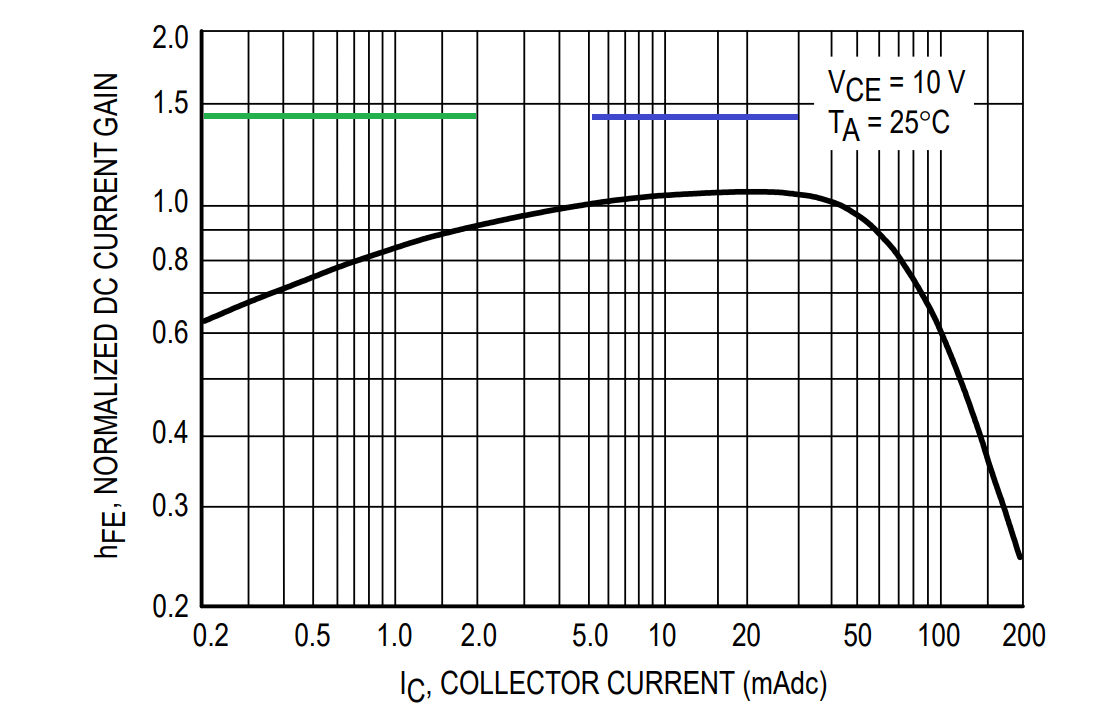
\includegraphics[width=0.6\textwidth, page=1]{ImagenesEjercicio2/hfe547b.png}
	\label{fig:hfe}
	\caption{Gráfico de HFE en función a la corriente de colector del BC547.}
\end{figure}
Lo que se busca es tener una corriente de colector tal que el hfe se encuentre en la zona azul, sin esta resistencia la corriente de colector probablemente se encontraría en la zona verde, lo cual no corresponde a un hfe estable.\\ 

El valor de $R_5$ se obtiene a partir de la siguiente ecuación:

\begin{align}
\frac{V_{BE}}{R_5}=I_{R5}\approx I_c
\end{align}
Para un valor de $13 \ mA$ corresponderá una resistencia de $56 \ \Omega$.

\subsubsection{Componentes de Protección}
Para la elección de estos componentes, se tuvo en cuenta la Ecuación (\ref{eq:Imaxfoldback}) para la cual, dado que se cuenta con dos grados de libertad, se fijó $R_a$ así la potencia disipada en corto-circuito no es de un valor muy elevado. Luego se tomó un valor para $R_c$, lo cual definió inequívocamente $R_b$. Para el cálculo de estos valores, se tuvo en cuenta que la máxima corriente ($2.5 \ A$) es suministrada únicamente cuando se regule a la tensión máxima. También se observó la pendiente de la curva de Foldback, la cual fue seleccionada para que cuando baje la tensión de regulación, aún tenga una corriente de salida máxima apreciable. Teniendo en cuenta esto, los valores seleccionados son los siguientes:
\begin{align}
R_a=0.56 \ \Omega  \ \ \ \ R_b=680 \ \Omega \ \ \ R_c=10 \ k\Omega \ \ \ I_{o-Max}=2.5 \ A \ \ \ I_{sc}= 1.34 \ A
\end{align}
Donde el valor de $I_{sc}$ queda fijado por la Ecuación (\ref{eq:Isc}).

\subsubsection{Diodo de Referencia}
El diodo zener elegido es el \href{https://d1d2qsbl8m0m72.cloudfront.net/en/products/databook/datasheet/discrete/diode/zener/bzx84b6v2lt116-e.pdf}{BZX84B6V2L},
debido a su reducida corriente de mantenimiento de $5 \ mA$.

Es primordial que el diodo se encuentre bien polarizado para proveer una referencia estable, para ello se fijó una corriente de zener de $I_Z =5.5 \ mA$, sabiendo que $V_Z=6.2 \ V$ y utilizando la Ecuación (\ref{eq:referencia}). De esta forma se llega a un valor $R_Z=120 \ \Omega$, siendo adicionalmente el valor de $V_2$ definido en la Sección (\ref{sec:fuentes}), mientras que el valor de $R_2$ es discutido en la Sección (\ref{sec:resdet}).

\subsubsection{Fuentes de Alimentación}
\label{sec:fuentes}
En cuanto a la elección de la fuente de alimentación, se buscó el $V_{1_{min}}$ tal que el sistema regule. Para esto, se pidió que el transistor de paso no se encuentre saturado en regulación, en otras palabras:
\begin{align}
V_{1_{min}}^{Transistor}=V_{CE_{sat}}+V_{O_{reg}}+V_{R_a}= 1.4 \ V+9 \ V +1.4 \ V \ =11.8 \ V
\end{align}

Otro punto de interés es la tensión a la salida del operacional, la cual no debe ser mayor a la de alimentación del mismo. Para obtener la variable en este nodo basta con seguir el circuito, observándose que:
\begin{align}
V_{1_{min}}^{Operacional}= V_o+V_{Ra}+2\cdot V_{BE} = 11.8 \ V
\end{align}

Luego, dado que este es el mínimo absoluto, se deja cierto margen de error para la tensión de saturación del transistor, al igual que para variaciones en la tensión de linea, las cuales pueden saturar a alguno de los transistores o al operacional. De esta forma se eligió un valor de $V_1=14 \ V$.

Finalmente para $V_2$ se fijó un valor que sea levemente mayor a la $V_Z$, tal que con el valor de resistencia $R_Z$ se encuentre polarizado correctamente. Es así que se obtuvo $V_2=7 \ V$.

\subsubsection{Resistencia circuito de detección}
\label{sec:resdet}
Dado que la salida en regulación depende directamente de la Ecuación (\ref{eq:vovz}), basta con definir un valor de $R_1$ tal que $V_o=9 \ V$, dado que la $R_1$ es un potenciómetro con el cual se varia la tensión de regulación. Así queda definido: $R_1= 10 \ k\Omega$ (potenciómetro) y $R_2=6.8  \  \Omega$

\subsection{Análisis de cargas}
En la búsqueda de la carga mínima, basta con una vez definida la máxima corriente y la máxima tensión de regulación, queda:

\begin{equation}
	R_{Lmin} = \frac{V_{Omax}}{I_{Omax}} = 3.6 \ \Omega
\end{equation}

Luego la máxima carga corresponde a $R_{LMax} = \infty$

\subsection{Análisis de Potencias Máximas}

\subsubsection{Amplificador Operacional}
\label{sec:opamppot}

Como ya se ha analizado en la Sección (\ref{sec:amp-error}), el amplificador operacional OP-284 cumple con la función de suministrar corriente al transistor de paso. Si bien esta corriente suministrada a la base del transistor es pequeña, el análisis en la Sección (\ref{sec:fuentes}) demuestra que la caída de potencial en el opamp es grande. Por esta razón se debe observar la potencia disipada para no quemar a este. Para el caso presente, se denota que el \href{https://www.alldatasheet.com/datasheet-pdf/pdf/49039/AD/OP284.html}{OP284} puede llegar hasta temperaturas de operación de $125 \ \degree C$. Asumiendo una temperatura ambiente de $40 \ \degree C$, y dejando un margen de seguridad de $15 \ \degree C$ en la temperatura del operacional, se calcula que la potencia máxima disipada por operacional es de $0.7 \ W$.
\begin{figure}[H]
\centering
	\includegraphics[width=0.6\textwidth, page=2]{ImagenesEjercicio2/Potencia.pdf}
	\caption{Circuito equivalente de potencias con $R_{\theta a-j} = 103 \ \frac{^o C}{W}$.}
	\label{fig:circuitopot}
\end{figure}

Para hallar la potencia máxima que disipa el amplificador operacional se deben considerar dos modos de funcionamiento de la fuente: en regulación y cuando la protección se encuentra activada. Para la primera, la tensión $V_0$ es constante, sin embargo, la corriente de salida es cada vez mayor, causando que el operacional entregue una corriente mayor a la base del transistor de paso. En este caso, y suponiendo que el transistor de protección esta totalmente apagado, se tiene que la corriente máxima que entrega el opamp es
\begin{equation}
	I_{opamp_{max}}|_{reg} = \frac{\frac{I_{o}}{\beta_{Q_2}}+\frac{V_{BE_{Q_2}}}{R_5}}{\beta_{Q_1}} =  \frac{\frac{2.5A}{100}+\frac{0.7V}{56\Omega}}{480} = 78uA
\end{equation}

Luego, utilizando la ley de mallas, se obtiene que
\begin{equation}
	V_{opamp_{max}}|_{reg} = V_o + I_{reg_{max}} \cdot R_a + V_{BE_{Q_2}} + V_{BE_{Q_1}} = 11.8V
\end{equation}

Por lo que la potencia máxima disipada por el operacional en regulación es
\begin{equation}
	P_{opamp_{max}}|_{reg} = 920.4uW
\end{equation}
siendo este un valor muy por debajo del máximo.

Por otro lado, cuando se activa la protección de Foldback, si bien la tensión es menor, el transistor de paso continua pidiendo corriente al operacional, mientras que a este se le suma el transistor de protección $T_P$. Se puede observar que, aunque la corriente $I_o$ decrezca, la corriente que pide $T_P$ es mediante su colector, por lo que no reduce en un factor de $\beta_p$ como sucedía con el transistor de paso, por lo que la corriente que se le pide al opamp es mucho mayor que en regulación, mientras que el peor caso se da cuando la carga tienda a cero.

Sin embargo, la tensión a la salida de la fuente regulada disminuye, por lo que también lo hará la tensión en el amplificador operacional, contrarrestando, pero no en su mayoría, el aumento de corriente. En la Sección \ref{sec:sim-pot} se analizó la curva de potencia disipada del operacional cuando la fuente se encuentra cortocircuitada, obteniendo una potencia máxima disipada de $P_{opamp_{max}}|_{cc} = 330 \ mW$ el cual se encuentra aún por debajo de la máxima potencia que puede disipar el amplificador operacional.

\subsubsection{Transistores}
\begin{figure}[H]
\centering
	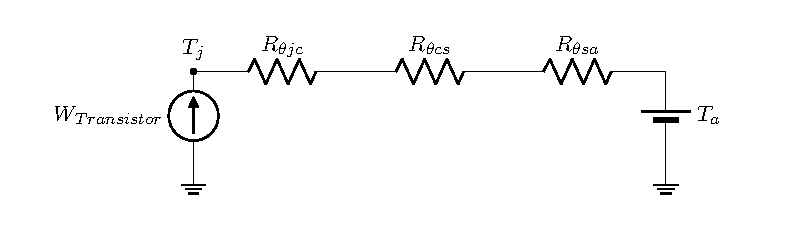
\includegraphics[width=0.6\textwidth, page=1]{ImagenesEjercicio2/Potencia.pdf}
	\caption{Circuito térmico para el cálculo de disipador del transistor.}
	\label{fig:circuitopottrans}
\end{figure}

\begin{equation}
\frac{T_j - T_a}{R_{\theta jc}+R_{\theta cs}+R_{\theta sa}} = P
\end{equation}

Asumiendo una temperatura ambiente de $40 \ \degree C$ y una temperatura máxima de juntura en funcionamiento de $140 \ \degree C$, $20 \ \degree C$ menor a la especificada por el fabricante, sabiendo que la $R_{\theta jc}$ es de $3.125 \ \frac{\degree C}{W}$, valiéndose del uso de una grasa siliconada de 0.002 pulgadas de espesor con una resistencia térmica de $204 \ \frac{\degree C \cdot inch}{W}$ y un área estándar de un empaquetado de TO-220 de $0.41\cdot 0.59 \ inch^2$, teniendo una $R_{\theta cs}$ de $1.6866 \ \frac{\degree C}{W}$ y asumiendo  una potencia disipada de $9.6 \ W$, levemente mayor a la máxima disipada, se obtiene
\begin{equation}
R_{\theta sa} = 4.57 \ \frac{\degree C}{W}
\end{equation}

\subsubsection{Diodos y Resistencias}
\begin{itemize}
	\item Para el diodo zener se obtiene que
	\begin{align}
		P_{z}=I_{z}^2\cdot r_z+I_z \cdot V_z = 34.4 \ mW
	\end{align}
	La máxima potencia capaz de disipar dicho diodo es de $250 \ mW$, por lo que este componente se encuentra en perfectas condiciones.

	\item Para $R_a$ es 
	\begin{align}
		P_{Ra}=I_{max}^2\cdot R_a+ = 3.5 \ W
	\end{align}
	Utilizando una $R_a$ de potencia.

	\item Para $R_5$ es
	\begin{align}
		P_{R5}=I_{R5}^2\cdot R_5 = 9.46 \ mW
	\end{align}
	la cual es una resistencia de $0.25 \ W$

	\item Para $R_2$ es
	\begin{align}
		P_{R2}=\frac{V_z^2}{R_2} = 57 \ mW
	\end{align}

	\item Finalmente, para $R_z$ se obtiene
	\begin{align}
		P_{Rz}=\frac{(V^- - V_z)^2}{R_z} = 5.33 \ mW
	\end{align}
\end{itemize}

\subsection{Rendimiento}

\subsection{Simulaciones}

\subsubsection{Respuesta en régimen transitorio de Regulación}
La respuesta transitoria del sistema se asemeja a la de un sistema de segundo orden. Cabe aclarar que los gráficos obtenidos de las simulaciones presentadas a continuación fueron realizados con una carga igual a la mínima que el sistema soporta.
\begin{figure}[H]
\centering
	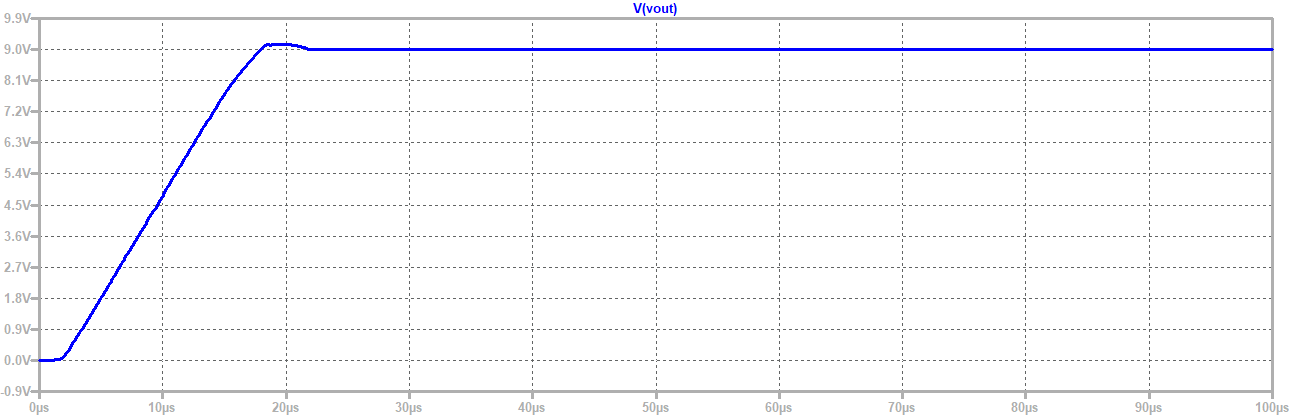
\includegraphics[width=1\textwidth]{ImagenesEjercicio2/transresp.png}
	\caption{Respuesta transitoria.}
	\label{fig:transitorioFuente}
\end{figure}

Es notable señalar, que el sobrepico del sistema alcanza $9.15 \ V$, lo cual representa un $1.6\%$ de desvío respecto de la tensión de regulación. También observar que el tiempo de establecimiento del sistema es aproximadamente $22 \ \mu s$.

Además, se simuló el circuito siendo afectado por ruido, con una frecuencia de $10 \ kHz$ y una amplitud de $0.5 \ V$. Estos valores fueron elegidos de forma tal que fuera apreciable la variación  durante el transitorio.
\begin{figure}[H]
\centering
	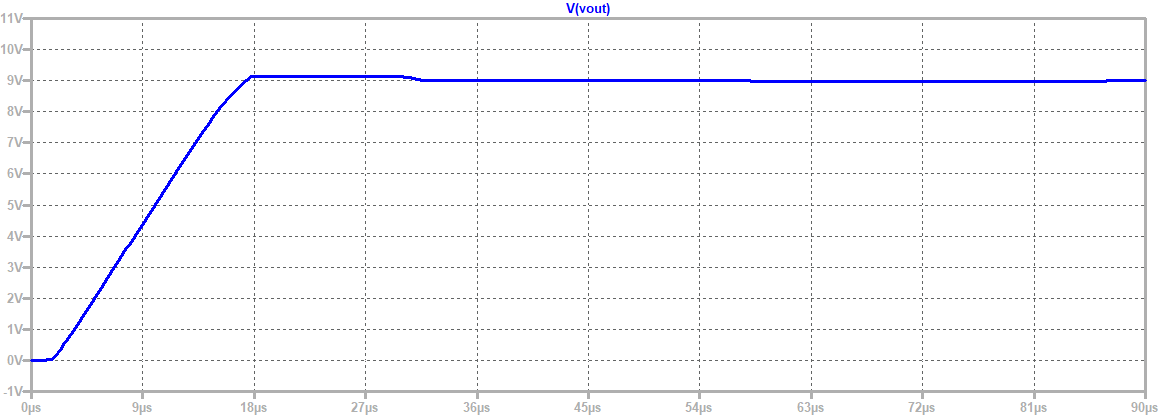
\includegraphics[width=1\textwidth]{ImagenesEjercicio2/transrespnoise.png}
	\caption{Respuesta transitoria con ruido.}
	\label{fig:transitorioFuentenoise}
\end{figure}

La Figura (\ref{fig:transitorioFuentenoise}) es similar a la (\ref{fig:transitorioFuente}) debido a la frecuencia del ruido. Aun así se puede apreciar una diferencia de las pequeñas oscilaciones generadas por el ruido en la tensión estabilizada en $9 \ V$. En cuanto a los parámetros del transitorio, el máximo sobrepico alcanzado es de $9.15 \ V$ y el tiempo de establecimiento es de aproximadamente $32 \ \mu s$.

\subsubsection{Respuesta en régimen permanente de Regulación}
En el caso del régimen permanente se ve la capacidad de mantener al tensión regulada en la salida. Dada la situación en que la señal no tenga ruido, la tensión regulada es de $9 \ V$ sin ningún tipo de variación.
\begin{figure}[H]
\centering
	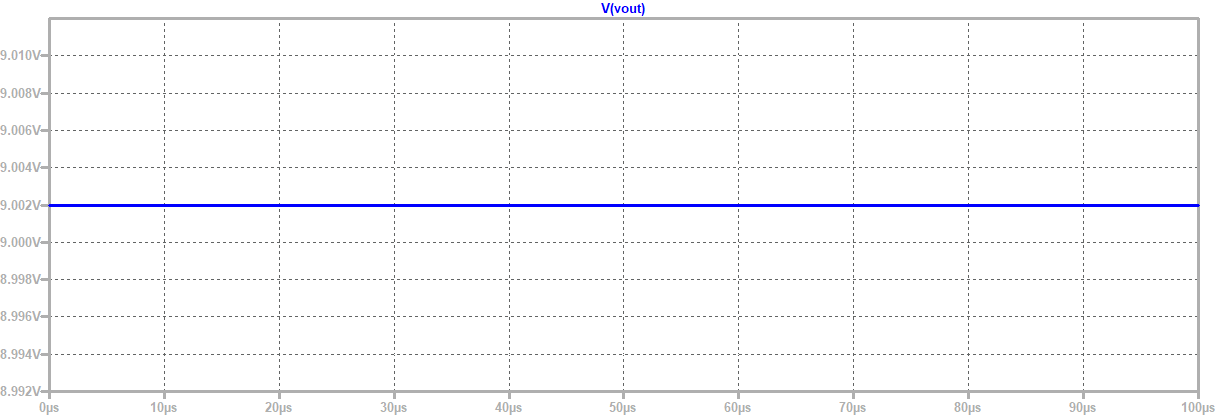
\includegraphics[width=1\textwidth]{ImagenesEjercicio2/permresp.png}
	\caption{Respuesta en régimen permanente.}
	\label{fig:permanenteFuente}
\end{figure}

A continuación, se presenta la respuesta del sistema frente a señales con distintos tipos de contaminación.

Para la primer prueba se ve la señal original, con la adición de una señal senoidal de $10 \ kHz$ de amplitud $0.5 \ V$. La salida es la siguiente:
\begin{figure}[H]
\centering
	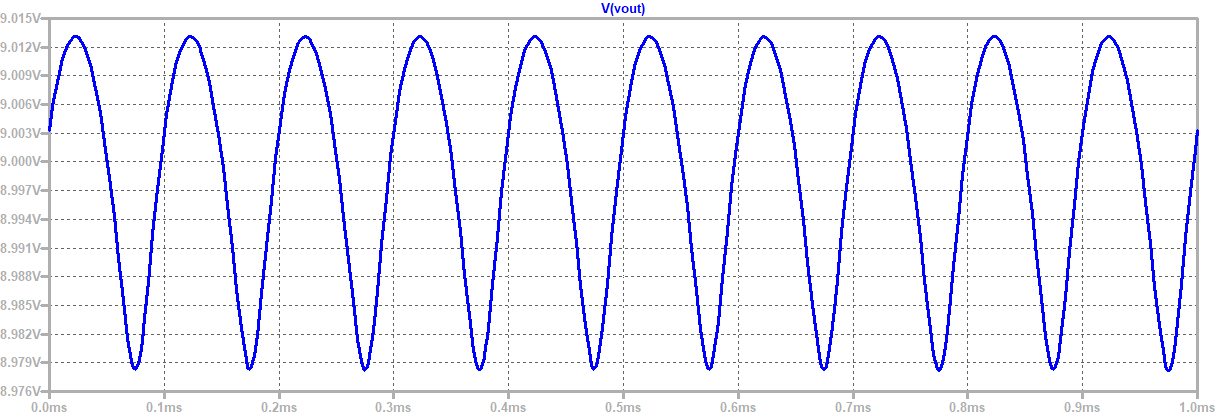
\includegraphics[width=1\textwidth]{ImagenesEjercicio2/permrespsine.png}
	\caption{Respuesta en régimen permanente con ruido senoidal.}
	\label{fig:permanenteFuentesine}
\end{figure}

Se puede ver que el desvío respecto de los $9 \ V$ es del $0.14\%$. Luego se agregó una señal triangular de frecuencia $50 \ Hz$ y amplitud unitaria.
\begin{figure}[H]
\centering
	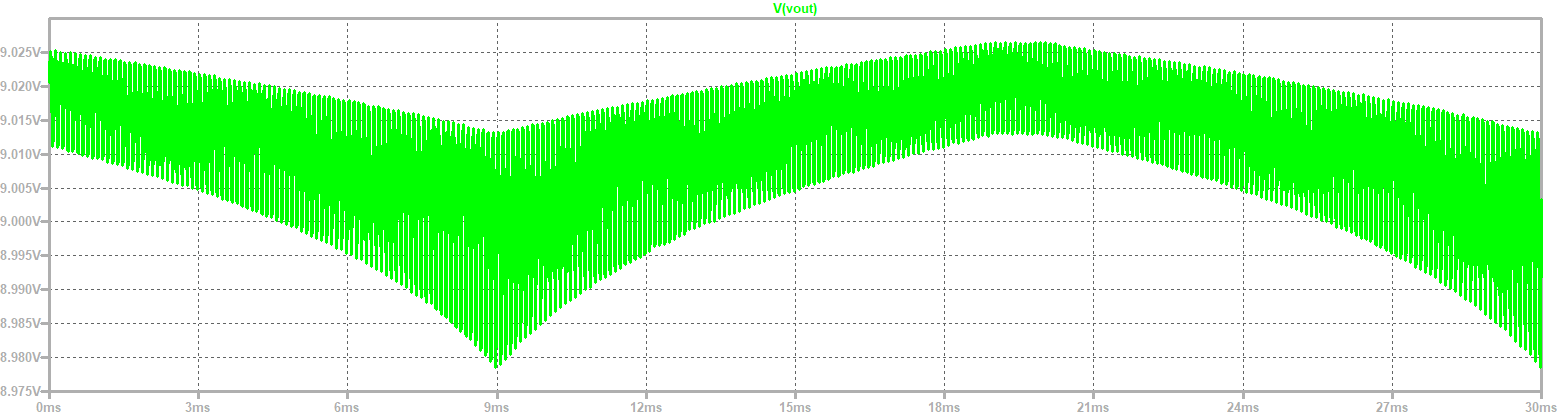
\includegraphics[width=1\textwidth]{ImagenesEjercicio2/permrespsinetri.png}
	\caption{Respuesta en régimen permanente con ruido senoidal y triangular.}
	\label{fig:permanenteFuentesinetri}
\end{figure}

Es notable que incluso con estas dos fuentes de ruido, de distinta amplitud y frecuencia, el sistema continúa regulando con un desvió no mayor del $0.24\%$.

\subsubsection{Respuesta en Frecuencia}

\subsubsection{Curva de Foldback}
La curva correspondiente al Foldback fue simulada y graficada como se ve a continuación:
\begin{figure}[H]
\centering
	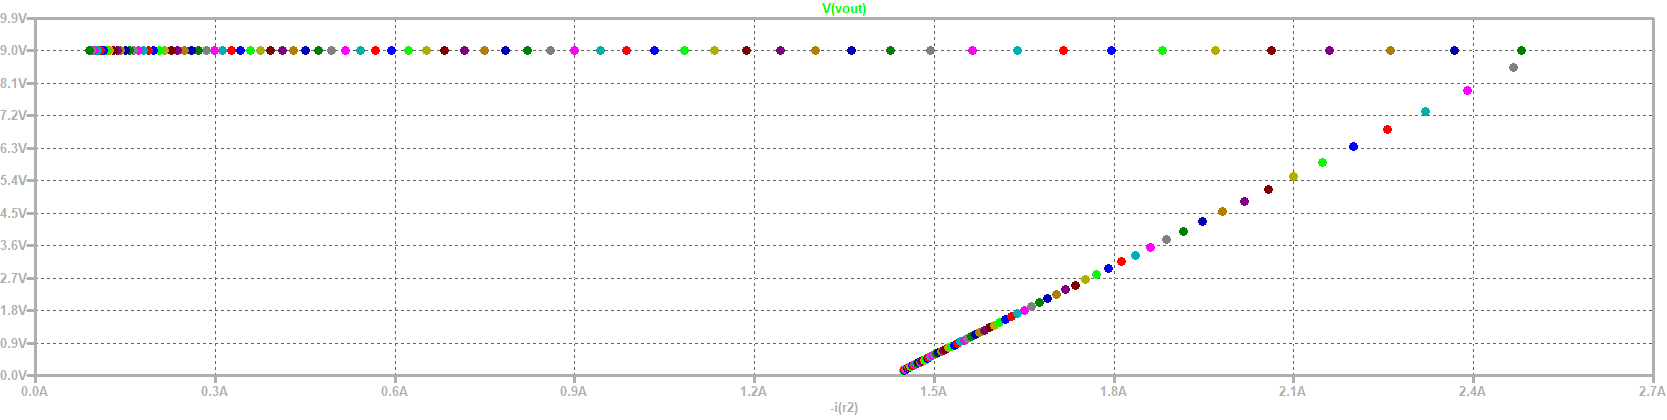
\includegraphics[width=1\textwidth]{ImagenesEjercicio2/curvefoldback.png}
	\caption{Curva de Foldback.}
	\label{fig:GraficoFOldbacki}
\end{figure}

Se puede apreciar que la máxima corriente es de $2.5 \ A$ como fue calculado, al igual que el valor de $I_{sc}$. Vale la pena mencionar que a medida que varíe la $R_1$, también lo hará la corriente máxima de salida acorde a la Ecuación (\ref{eq:Imaxfoldback}).

\subsubsection{Impedancia de Salida}
La impedancia de salida fue simulada y graficada:
\begin{figure}[H]
\centering
	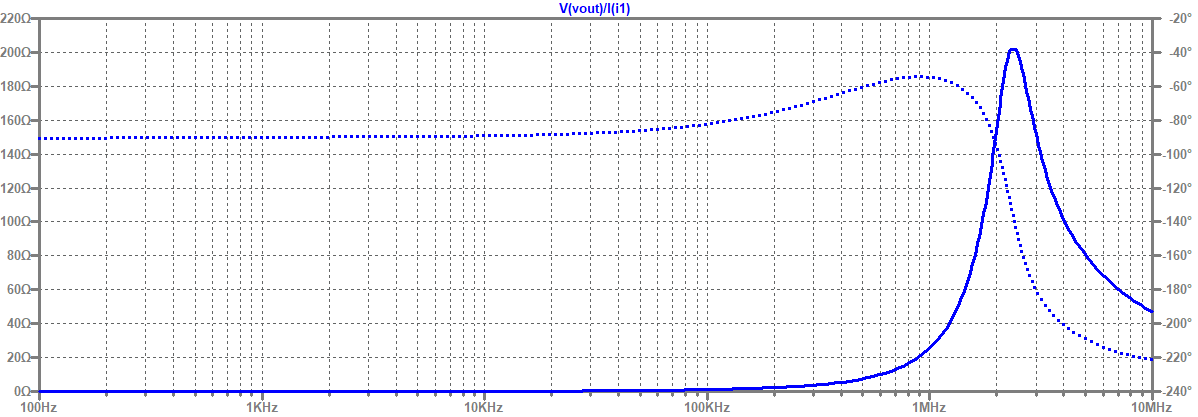
\includegraphics[width=1\textwidth]{ImagenesEjercicio2/zoutspice.png}
	\caption{Impedancia de salida.}
	\label{fig:zout}
\end{figure}

Se observa que la impedancia de salida es baja para la mayor parte del espectro, sin superar los $220 \ \Omega$.

\subsubsection{Potencias}
\label{sec:sim-pot}
En esta sección se simularon las curvas de potencias sobre los componentes al variar la carga del circuito.

\begin{itemize}
\item Diodo Zener: 
Se puede ver que la máxima potencia disipada corresponde a la mínima carga, siendo esta de $37 \ mW$ lo cual no es un problema para dicho diodo.
\begin{figure}[H]
\centering
	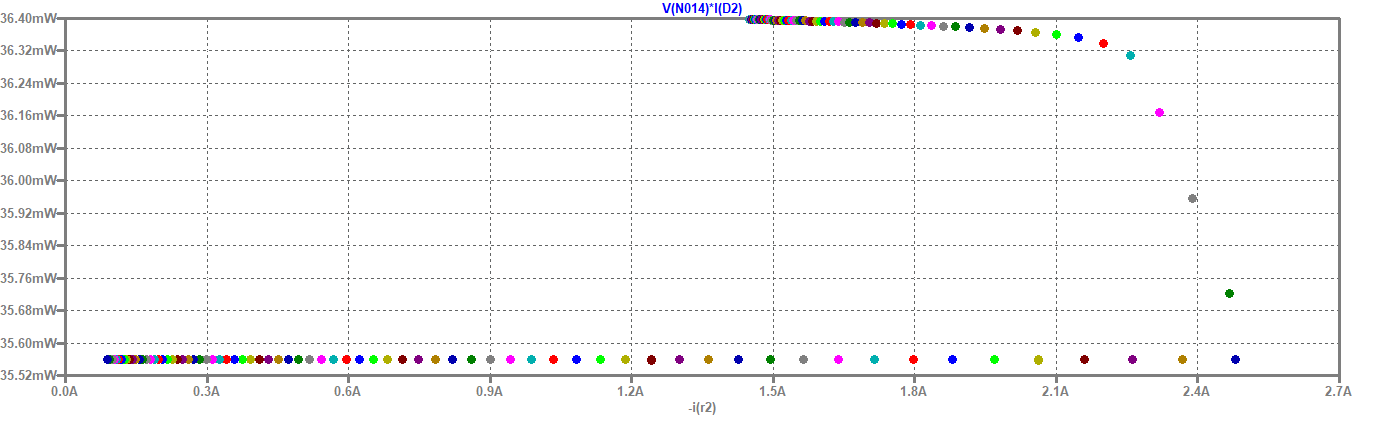
\includegraphics[width=1\textwidth]{ImagenesEjercicio2/potzener.png}
	\caption{Potencia sobre el zener.}
	\label{fig:potzener}
\end{figure}

\item BC547C Darlington: La máxima potencia es de $330 \ mW$, lo cual no es un problema para dicho transistor. Al igual que la anterior curva se observa un aumento considerable una vez que se activa el Foldback, pero aun en la zona de operación tiene una pendiente.
\begin{figure}[H]
\centering
	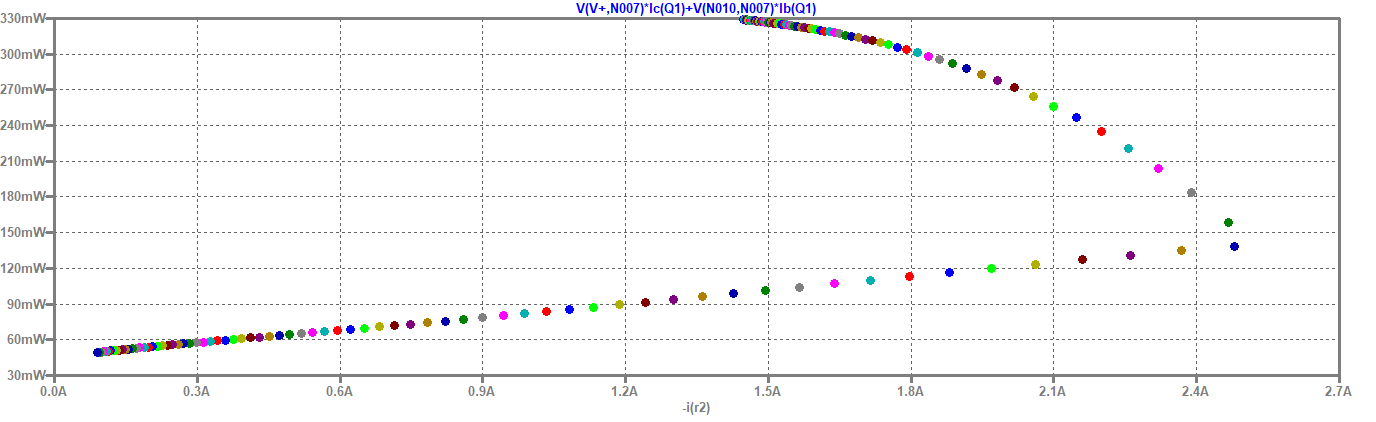
\includegraphics[width=1\textwidth]{ImagenesEjercicio2/potbc547.png}
	\caption{Potencia sobre el BC547C del darlington.}
	\label{fig:potbc547}
\end{figure}

\item $R_a$: La potencia máxima disipada corresponde a $3.5 \ W$, lo cual es esperado dado que es $R_a\cdot I_{max}^2$. 
\begin{figure}[H]
\centering
	\includegraphics[width=1\textwidth]{ImagenesEjercicio2/potra.png}
	\caption{Potencia sobre la $R_a$.}
	\label{fig:potra}
\end{figure}

\item TIP31C: La potencia sobre estos transistores de potencia es de $9 \ W$, lo cual indica que un disipador debe ser utilizado para su correcto funcionamiento.
\begin{figure}[H]
\centering
	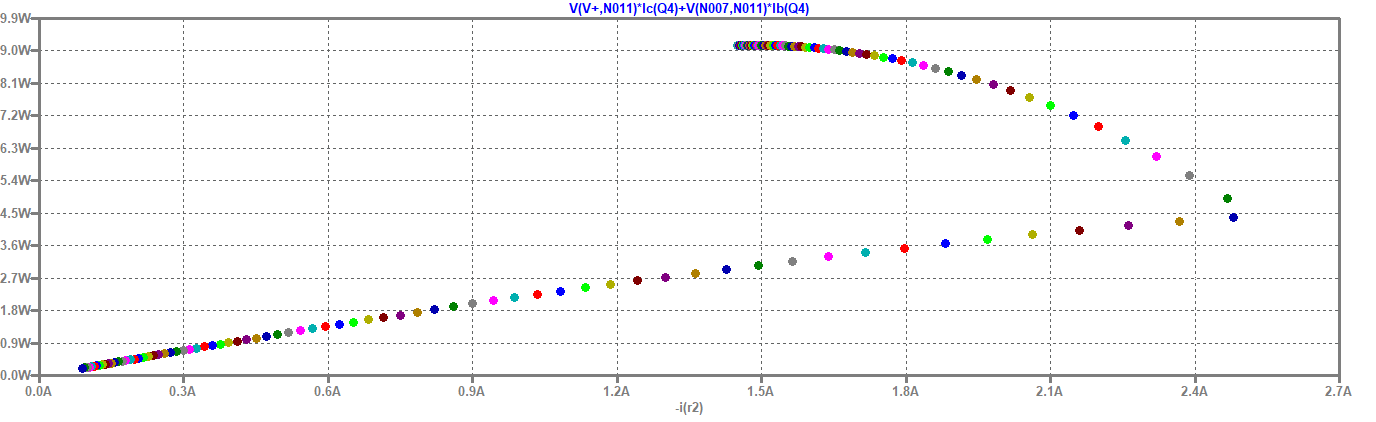
\includegraphics[width=1\textwidth]{ImagenesEjercicio2/pottip31c.png}
	\caption{Potencia sobre el TIP31C.}
	\label{fig:pottip31}
\end{figure}

\item BC547 Protección: Se debe notar que el transistor no consume potencia, sino hasta el momento en el cual se activa, alcanzando un limite de $60 \ mW$.
\begin{figure}[H]
\centering
	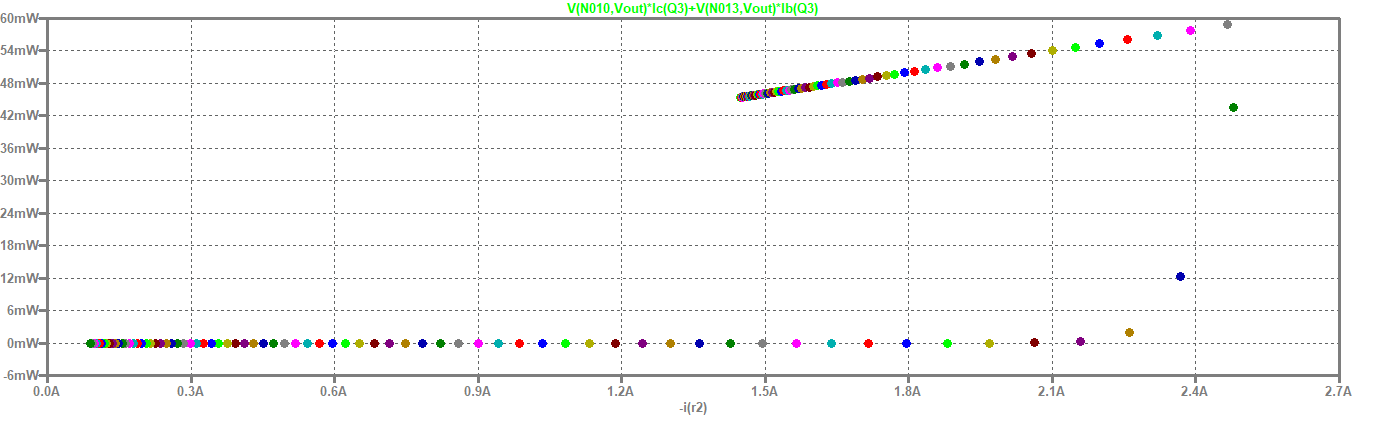
\includegraphics[width=1\textwidth]{ImagenesEjercicio2/potprot.png}
	\caption{Potencia sobre el BC547C de la protección.}
	\label{fig:potbc547prot}
\end{figure}

\item Operacional: Para este se observa que la máxima potencia corresponde a $330 \ mW$ al tener una carga nula. Vale la pena mencionar que, al medir la potencia en LTSpice, dicho programa considera las corrientes de alimentación.
\begin{figure}[H]
\centering
	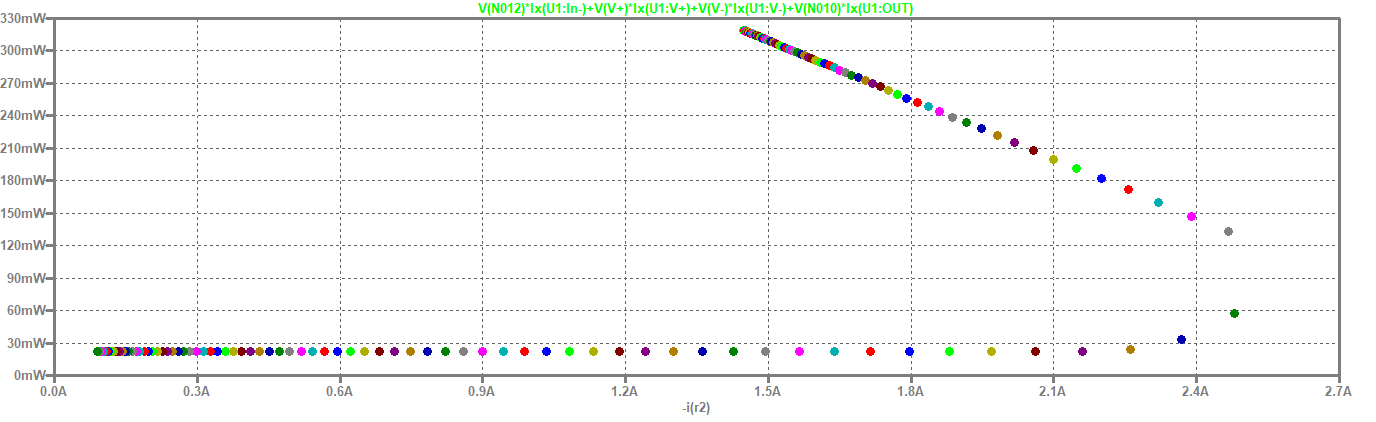
\includegraphics[width=1\textwidth]{ImagenesEjercicio2/potopamp.png}
	\caption{Potencia sobre el operacional.}
	\label{fig:potop}
\end{figure}

\item Carga: Se observa que el crecimiento es lineal hasta la activación de la protección y luego sigue la curva del Foldback, teniendo una potencia máxima de $22.5 \ W$.
\begin{figure}[H]
\centering
	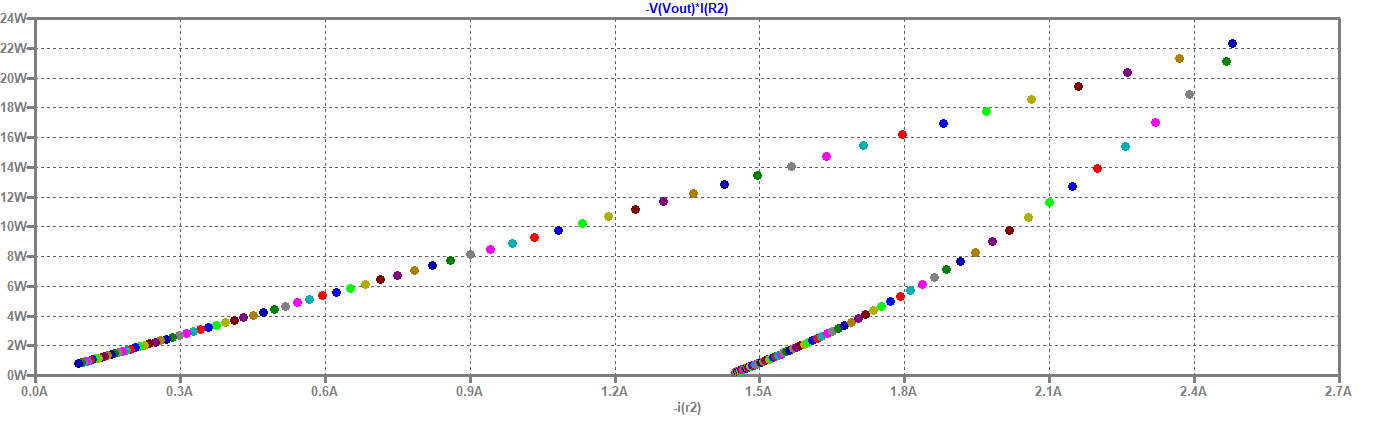
\includegraphics[width=1\textwidth]{ImagenesEjercicio2/potload.png}
	\caption{Potencia sobre la carga.}
	\label{fig:potload}
\end{figure}
\end{itemize}

\subsection{Conclusiones}


\end{document}